\section{Technical Overview}
\label{design}

\begin{figure}[th!]
        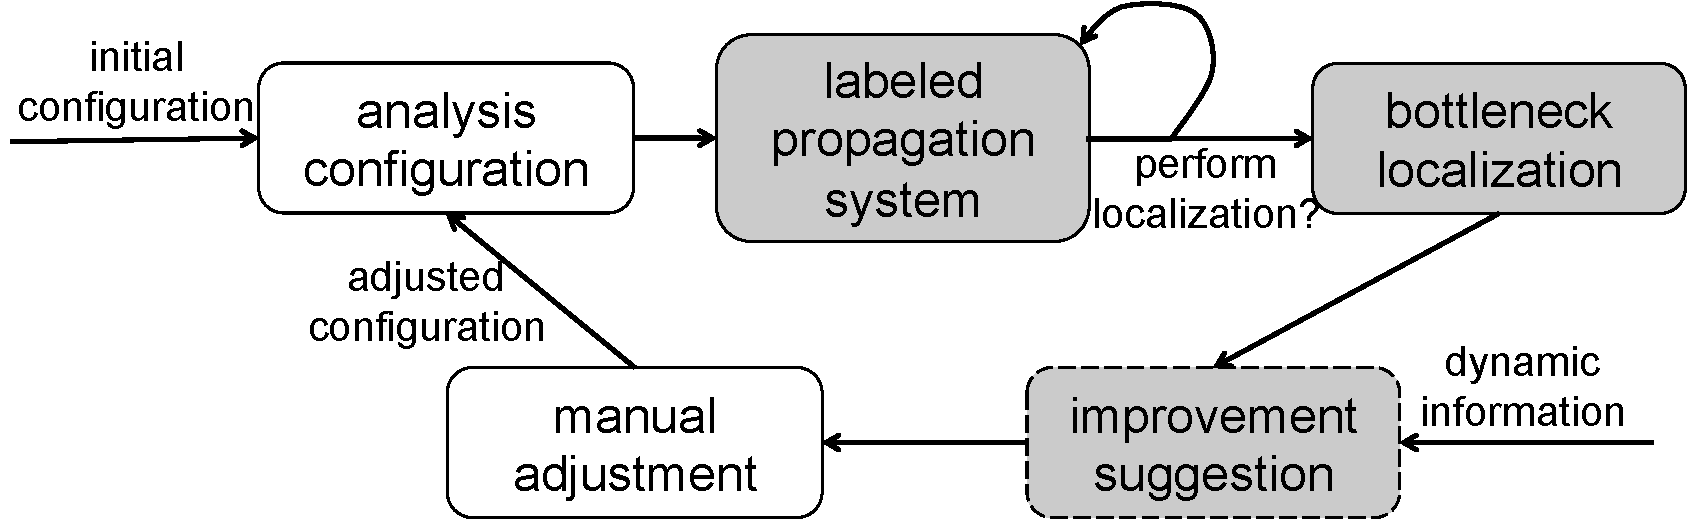
\includegraphics[width=\columnwidth]{overview}
\caption{\textmd{Root-cause localization process overview.}}
\label{fig:overview}
\end{figure}

%\subsection{Overview}

Figure \ref{fig:overview} summarizes the root-cause localization process with the support of our automated techniques. We discuss the steps comprising the process in the following.

We first run the static analysis in its initial context sensitivity configuration, which may lead to performance and/or precision issues. To monitor the behavior of the analysis, we run it in \emph{diagnostic} mode by instrumenting the propagation system with labels, the result being a \emph{labeled propagation system} that keeps track of the history of point-to propagations by labeling the origins of points-to relations. We avoid from the common situation that the analysis crashes (i.e., running out of time/space budgets), and so the metadata for root-cause localization is lost, by obtaining snapshots of the analysis' state periodically.

Later, in Section \ref{Se:RootCause}, we describe and motivate our heuristics to determine whether the observed propagation behavior is anomalous. Intuitively, an anomaly is flagged if a given variable or reference property, collectively referred to as \emph{program pointers}, is associated with a large points-to set, and the label corresponding to the pointer propagates to many other pointers within a small number of evaluations of the propagation system. Here is where the labels come into play, in recording the transitive propagation of abstract objects across pointers. Our localization algorithm ranks the results by order of their impact on precision, thereby reflecting how likely they are to be among the root causes for imprecision.

The optional remediation step, where suggestions for improvement are provided, accepts as input (i) the candidate root causes, (ii) a set of context sensitivity policies, as well as (iii) one or more dynamic execution traces of the program. The significance of the dynamic traces is in providing fully precise points-to information, such that the effect of different sensitivity policies can be evaluated.

Intuitively, the remediation process maps between the root causes identified statically and the concrete points in the trace $t$, and simulates the effect of different sensitivity policies atop $t$. Given for example statement $\ell\colon {\sf y=x[p]}$ in method $m$ as the root cause, the first step is to simulate the least precise treatment of $\ell$ by merging together concrete points-to information from all its occurrences in $t$. What follows is an iterative process, wherein different context sensitivity, and combinations thereof, are applied, and their effects are simulated. A suggestion is output for $\ell$ to utilize a certain combination $C$ of context sensitivity if (i) $C$ partitions the points-to set of ${\sf x[p]}$ effectively, and (ii) more involved combinations are only negligibly better.

The final step, following the automated techniques, is for the user (i.e., either the analysis designer or an end user capable of configuring the analysis) to manually adjust the analysis configuration based on the localization results and/or the improvement suggestions. Upon doing so, the analysis can be rerun under the adjusted configuration to observe if the performance and/or precision issues have been resolved. The same process can be performed iteratively to locate all the root causes, thereby leading to a specialized analysis configuration that meets the performance/precision requirements of the user at hand.

In the next two sections, we dive into the details of the two main algorithms: root-cause localization and improvement suggestion. We discuss each in turn.

\begin{comment}
\begin{algorithm}[th!]
\floatname{algorithm}{Proc}
	\begin{algorithmic}[1]
		{
			\renewcommand{\algorithmicrequire}{\textbf{Input:}}
			\renewcommand{\algorithmicensure}{\textbf{Output:}}
			\REQUIRE {\tt config}: analysis configuration
			\REQUIRE {\tt i}: evaluation interval
			\ENSURE {\tt R}: set of root causes
			\STATE {\tt sys} $\leftarrow$ initialize propagation system with {\tt config}
			\WHILE{({\tt c} $\leftarrow$ next constraint in {\tt sys}) {\tt != NULL} //fixed-point has not been reached} 
			%\STATE {\tt pts} $\leftarrow$ points-to propagation on {\tt c}
			\FOR{each points-to assignment {\tt v1 = v2} from {\tt c}}
			\STATE {\tt pts\textsubscript{v1}= pts\textsubscript{v1} $\bigcup$ pts\textsubscript{v2}} //points-to propagation
			\STATE {\tt l\textsubscript{v1} = l\textsubscript{v1} $\bigcup$ l\textsubscript{v2} $\bigcup$ \{v2\}} //label propagation
			\ENDFOR
			\IF{{\tt (k $\leftarrow$ No. of evaluations) mod i = 0}}
			\STATE  grow $\leftarrow$ points-to size growth in past {\tt i} evaluations
			\IF{grow > threshold //to perform localization when the growth rate is high}
			\STATE g $\leftarrow$ intermediate points-to graph with labels //do not require a complete graph
			\FOR{each pointer key node {\tt n} in {\tt g}}
			\STATE impact\textsubscript{n} $\leftarrow$ compute the impact of {\tt n} on {\tt g}
			\ENDFOR
			\STATE V $\leftarrow$ nodes with high impacts
			\RETURN
			\ENDIF
			\ENDIF
			\ENDWHILE
		}
	\end{algorithmic}
	\caption{Root-cause localization workflow.}
	\label{alg:localization}
\end{algorithm}
\end{comment}

\begin{algorithm}[th!]
\floatname{algorithm}{Proc}
	\begin{algorithmic}[1]
		{
			\renewcommand{\algorithmicrequire}{\textbf{Input:}}
			\renewcommand{\algorithmicensure}{\textbf{Output:}}
			\REQUIRE {\tt config}: analysis configuration
			\REQUIRE {\tt i}: evaluation interval
			\ENSURE {\tt R}: set of root causes
			\STATE {\tt sys} $\leftarrow$ initialize propagation system with {\tt config}
			\WHILE{({\tt c $\leftarrow$ sys.<next constraint>) != NULL}} 
			%\STATE {\tt pts} $\leftarrow$ points-to propagation on {\tt c}
			\FOR{each assignment {\tt v1 = v2} from {\tt c}}
			\STATE {\tt pts\textsubscript{v1}= pts\textsubscript{v1} $\bigcup$ pts\textsubscript{v2}} {\it //points-to propagation}
			\STATE {\tt l\textsubscript{v1} = l\textsubscript{v1} $\bigcup$ l\textsubscript{v2} $\bigcup$ \{v2\}} {\it //label propagation}
			\ENDFOR
			\IF{{\tt (k $\leftarrow$ \# of evaluations) mod i = 0}}
			\STATE  {\tt grow $\leftarrow$} points-to size growth in past {\tt i} evaluations
			\IF{grow > threshold}
			\STATE {\tt g $\leftarrow$} intermediate static labelled points-to graph
			\FOR{each pointer node {\tt n} in {\tt g}}
			\STATE {\tt impact\textsubscript{n} $\leftarrow$} compute the impact of {\tt n} on {\tt g}
			\ENDFOR
			\STATE {\tt R $\leftarrow$} high impact nodes
			\RETURN
			\ENDIF
			\ENDIF
			\ENDWHILE
		}
	\end{algorithmic}
	\caption{Root-cause localization workflow.}
	\label{alg:localization}
\end{algorithm}

\section{Root-cause Localization}\label{Se:RootCause}

We first explain, more technically, how the labeled propagation system is implemented. We then move to a description of our indicators, based on the labels, whether an anomalous propagation behavior is taking place. The overall workflow of root-cause localization is shown in Procedure \ref{alg:localization}.

\subsection{Labeled Propagation System}

A propagation system for the points-to analysis solves the constraints to reach a fixpoint, propagating the points-to relations of the variables and reference properties in the program. A majority of the constraints that exist in the propagation system are assignments. For example, to process an invoke instruction, the generated constraints include assignments from the actual arguments to the formal parameters, from the callee's return values to the left-hand side variable of the invoke instruction, etc. 

We assume a subset-based (aka inclusion-based) propagation system \cite{andersen1994program}, which means that the system solves a constraint that assigns a program pointer {\tt v1} to another pointer {\tt v2} by adding the points-to set of {\tt v1} to that of {\tt v2}. In a standard propagation system, there is no provenance. The points-to set associated with a pointer may be the result of direct or transitive assignments, and there is no telling in general how it evolved to its current state. Such information is critical, however, to identify root causes, since frequent assignments involving an inaccurate points-to set may pollute the overall precision of the points-to solution as depicted in Figures \ref{fig:pts-growth} and \ref{fig:pts-distribution}.

To address this loss of information, in our labeled propagation system, each constraint that assigns the values of {\tt v2} to {\tt v1} results in not only the changes to {\tt v1}'s points-to relations but also a label {\tt v2} associated with the points-to set of {\tt v1}, indicating that (some of) the points-to relations of {\tt v1} were propagated through {\tt v2} (lines 3-6 in Procedure \ref{alg:localization}). As an example, in WALA\footnote{http://wala.sourceforge.net/wiki/index.php/Main\_Page} intermediate representation (IR), which is in SSA form \cite{Cytron:1991:ECS:115372.115320}, the statement at line 5 in Figure \ref{fig:jquery-modified} reduces to (a) {\tt v\textsubscript{tmp} = source[name]} and (b) {\tt target[name] = v\textsubscript{tmp}}, where {\tt v\textsubscript{tmp}}, {\tt source}, {\tt target} and {\tt name} are all local variables of the function.  

For the property read instruction (a), the analysis would first query the points-to set of {\tt source}, {\tt P\textsubscript{source}}, and the points-to set of {\tt name}, {\tt P\textsubscript{name}}. The pairs of each element in {\tt P\textsubscript{source}} and {\tt P\textsubscript{name}} (e.g., {\tt p\textsubscript{source\_i}.p\textsubscript{name\_j}}) are returned as the results of looking up the reference properties of {\tt source[name]}. Note that the values of {\tt name} iterate over all the property names of {\tt source}, which in practice are the large set of function names loaded in {\it jQuery}. This ultimately results in a large points-to set for {\tt v\textsubscript{tmp}} due to multiple assignments from various reference properties. We retain all these reference properties (e.g., {\tt p\textsubscript{source\_i}.p\textsubscript{name\_j}}) as labels attached to the points-to set of {\tt v\textsubscript{tmp}}. 

For the property write instruction (b), the analysis similarly looks up the reference properties of {\tt target[name]} (e.g., {\tt p\textsubscript{target\_i}.p\textsubscript{name\_j}}) and adds the points-to relations of {\tt v\textsubscript{tmp}} to each of these reference properties, resulting in an overly approximated points-to set for each function name in {\it jQuery}. We retain both {\tt v\textsubscript{tmp}} and the existing transitive labels from {\tt v\textsubscript{tmp}} (e.g., {\tt p\textsubscript{source\_i}.p\textsubscript{name\_j}}) in the points-to set of each reference property of {\tt target[name]}.

In addition to tracking the set of labels that are immediately or transitively propagated to the points-to set of a given pointer, we generate a {\it propagation-history graph} for the points-to set of that pointer, which organizes the points-to propagation history into a hierarchical structure. Intuitively, a node in the propagation-history graph is a program pointer that has bearing on the specific points-to set. An edge from node {\tt n\textsubscript{1}} to another node {\tt n\textsubscript{2}} represents that the points-to set of {\tt n\textsubscript{2}} was explicitly added to that of {\tt n\textsubscript{1}}. The entry points of the graph are the program pointers whose points-to sets are directly propagated into the corresponding points-to set. 

For the same example in Figure \ref{fig:jquery-modified}, the propagation-history graph for the points-to set of {\tt v\textsubscript{tmp}} consists of all the reference properties of {\tt source[name]} as entry points. {\tt v\textsubscript{tmp}} is the entry point of the propagation-history graph for the points-to set of each reference property of {\tt target[name]} (e.g., {\tt p\textsubscript{target\_i}.p\textsubscript{name\_j}}), while there also are edges from {\tt v\textsubscript{tmp}} to the properties of {\tt source[name]}.

\begin{figure}[th!]
        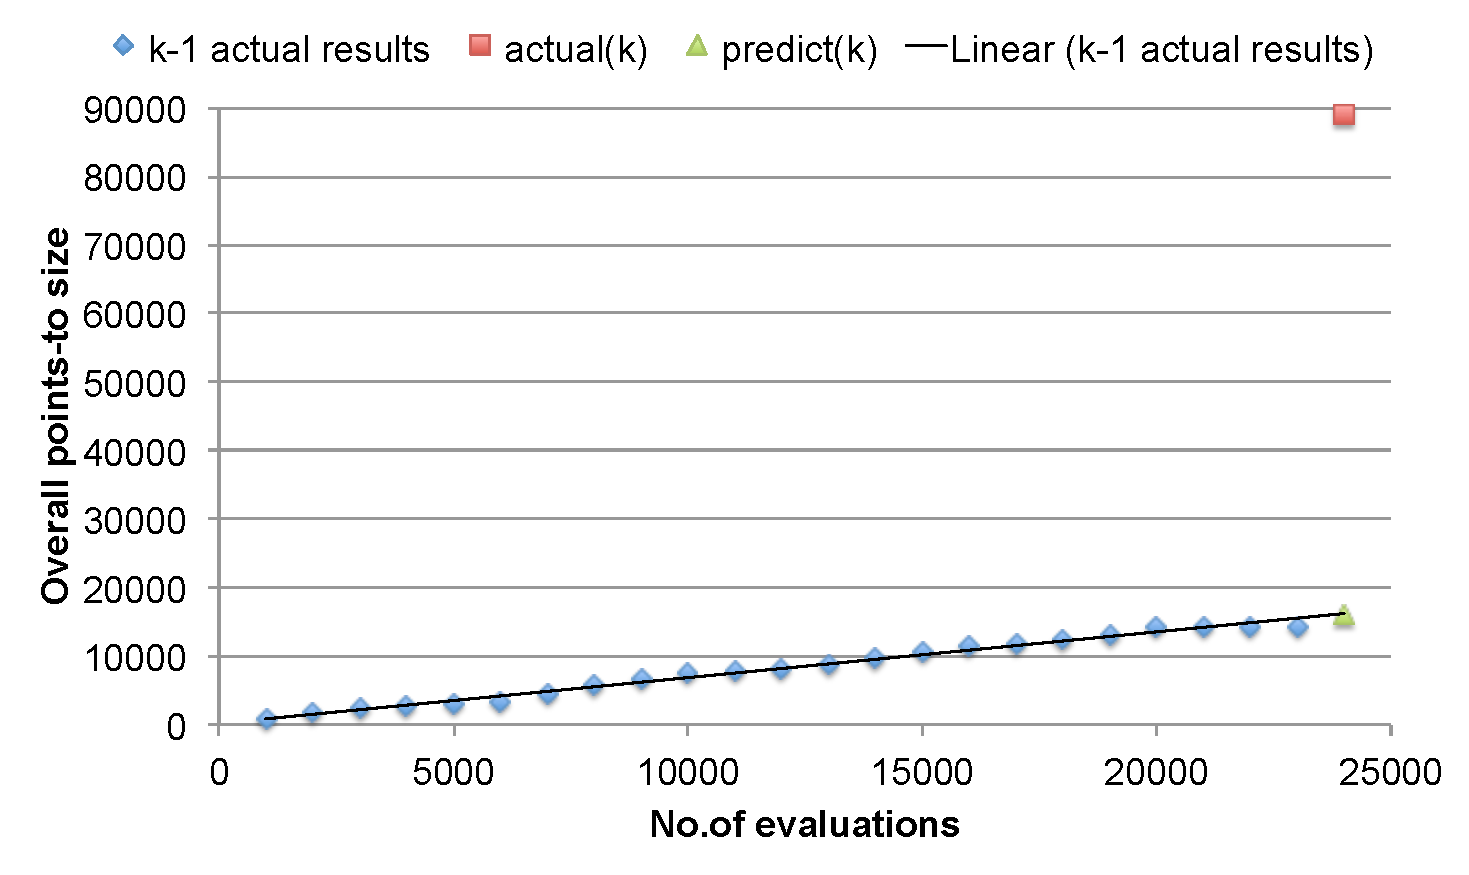
\includegraphics[width=\columnwidth]{linear}
\caption{\textmd{Prediction via linear regression.}}
\label{fig:linear}
\end{figure}

As motivated above, during the propagation process, the labeled system is paused regularly upon completing cycles of {\tt i} evaluations, for a fixed value of {\tt i} (line 7 in Procedure \ref{alg:localization}). We base our analysis of root causes of impracticality on the resulting intermediate states.

Specifically, we count the total number of points-to relations (i.e., edges) in the intermediate points-to graph for the {\tt k\textsubscript{th}} pause (i.e., after {\tt n$\times$k} evaluations), {\tt actual(k)}. We then compare the value of {\tt actual(k)} with the value of {\tt predict(k)} to decide whether to perform root-cause localization. 

For meaningful comparison, we utilize the results from the previous {\tt k-1} pauses in performing linear regression analysis to find the fitted line {\tt y = intercept + slope $\times$ x}, where {\tt x} is the number of evaluations and {\tt y} is the total number of points-to relations. The number of points-to relations of the {\tt k\textsubscript{th}} pause can then be predicted: {\tt predict(k) = intercept + slope $\times$ kn}. If {\tt actual(k) > 110\% $\times$ predict(k)}, then we decide to perform the root-cause localization at the {\tt k\textsubscript{th}} pause; otherwise, we continue the points-to analysis under the labeled propagation system. 

Figure \ref{fig:linear} shows this prediction model when running the 0-1-CFA analysis on a {\it jQuery} application. The analysis is paused every 1000 evaluations and the fitted line in Figure \ref{fig:linear} is calculated from the results of the first 23 pauses (i.e., 1000 to 23,000 evaluations). The predicted total points-to edges at the 24,000 evaluations is 16,234, while {\tt actual(24)} is 88,857, significantly passing the threshold to perform root-cause localization. This prediction model can capture the ``jump'' phase of the points-to analysis shown in Figure \ref{fig:pts-growth}, which is important to localize the root causes accurately. 

If localization is performed too early, the over-approximate results may not have surfaced yet. If localization is performed late during the analysis, then the over-approximate results due to the root causes may have polluted a large portion of the overall points-to results, making it difficult to identify the root causes of imprecision. Moreover, the evaluation interval to pause the analysis, {\tt i}, as well as the decision threshold, may be tuned based on the budget and goals of root-cause localization.

%During the progress, the label propagation system is paused periodically. The intermediate results are used to decide whether bottleneck localization is performed, using the predicted value of linear regression. A linear regression is predicted based on the {\tt k-1} pauses. If the actual value of the {\tt k}'s pause is greater than 110\% of the predicted value, we determine that the analysis may have entered the ``jump" period shown in Figure \ref{fig:pts-growth} and the bottleneck localization is performed.

\subsection{Identifying Root Causes for Divergence}

When performing root-cause localization, we use the intermediate points-to graph and the associated labels to identify possible root causes (line 10 in Procedure \ref{alg:localization}). For each variable or reference property {\tt v}, we count (i) its points-to size, {\tt |P\textsubscript{v}|}, as well as (ii) its number of occurrences as labels in the points-to sets of other variables and/or reference properties, {\tt |L\textsubscript{v}|}. {\tt |L\textsubscript{v}|} measures how widely {\tt v} reaches within the propagation system, and {\tt |P\textsubscript{v}|} measures if the impact of its wide reach is significant. We therefore use the scoring heuristic {\tt S\textsubscript{v}=|P\textsubscript{v}|$\times$|L\textsubscript{v}|} as a measurement of the possibility of {\tt v} being the root cause (lines 11-13 in Procedure \ref{alg:localization}). 

The root-cause localization stage reports a set of variables as root causes in descending order of their scores. For example, {\tt v\textsubscript{tmp}}, the result of the property read instruction at line 5 in Figure \ref{fig:jquery-modified}, achieves an extremely high score (73,950) with {\tt |P\textsubscript{v\textsubscript{tmp}}|=150} and {\tt |L\textsubscript{v\textsubscript{tmp}}|=493} when localization is performed after 24,000 evaluations. Its score is 75-times higher than the variable with the second highest score (990), rendering it the only root-cause candidate for imprecision of the 0-1-CFA analysis for this {\it jQuery} application. We report the variables and/or reference properties whose scores are at least half the highest score as {\it candidate (or suspicious) root causes}.

%We then assign score to each variable and/or reference property by calculating (i) $\times$ (2). The higher score indicates the variable is more likely to be analysis bottlenecks. We report the variables with scores great than half of the one with the highest scores.
\begin{comment}
\begin{algorithm}[th!]
\floatname{algorithm}{Procedure}
	\begin{algorithmic}[1]
		\renewcommand{\algorithmicrequire}{\textbf{Input:}}
		\renewcommand{\algorithmicensure}{\textbf{Output:}}
		\REQUIRE {\tt R = \{r\textsubscript{1}, ..., r\textsubscript{n}\}}: root causes
		\REQUIRE: {\tt t}: dynamic trace
		\ENSURE {\tt <V, S>=\{(r\textsubscript{1}, s\textsubscript{1}),...,(r\textsubscript{n}, s\textsubscript{n})\}}: suggestions
		\STATE G $\leftarrow$ taking {\tt t} as input, create a set of dynamic points-to graphs with different context sensitivity policies //some operations from Procedure 3 may be moved here
		\FOR{each {\tt r\textsubscript{i}} $\in$ {\tt R}}
		\STATE A\textsubscript{<r\textsubscript{i}, G>} $\leftarrow$ $\emptyset$ 
		\FOR{each {\tt g\textsubscript{j}} $\in$ {\tt G}}
		%\STATE |pts\textsubscript{(r, g)}| $\leftarrow$ query {\tt r}'s total points-to size in {\tt g}
		%\STATE |cs\textsubscript{(r, g)}| $\leftarrow$ query number of calling contexts for {\tt r} in {\tt g}
		\STATE a\textsubscript{<r\textsubscript{i}, g\textsubscript{j}>} $\leftarrow$ query {\tt r\textsubscript{i}}'s total points-to size in {\tt g\textsubscript{j}} and measure its accuracy corresponding to {\tt g\textsubscript{j}}'s context sensitivity policy
		\STATE A\textsubscript{<r\textsubscript{i}, G>} = A\textsubscript{<r\textsubscript{i}, G>} $\bigcup$ \{a\textsubscript{<r\textsubscript{i}, g\textsubscript{j}>}\}
		\ENDFOR
		\STATE a\textsubscript{<r\textsubscript{i}, g>} $\leftarrow$ min(A\textsubscript{<r\textsubscript{i}, G>}) //pick the dynamic points-to graph on which r\textsubscript{i} is the most accurate
		\STATE <V, S> = <V, S> $\bigcup$ \{<r\textsubscript{i}, g's context sensitivity>\}
		\ENDFOR
	\end{algorithmic}
	\caption{Improvement suggestion workflow.}
	\label{alg:suggestion}
\end{algorithm}
\end{comment}

\begin{algorithm}[th!]
\floatname{algorithm}{Proc}
	\begin{algorithmic}[1]
		\renewcommand{\algorithmicrequire}{\textbf{Input:}}
		\renewcommand{\algorithmicensure}{\textbf{Output:}}
		\REQUIRE {\tt R = \{r\textsubscript{1}, ..., r\textsubscript{n}\}}: root causes
		\REQUIRE {\tt t}: dynamic trace
		\REQUIRE {\tt CS}: context sensitivity policies
		\ENSURE {\tt <V, S>=\{(r\textsubscript{1}, s\textsubscript{1}),...,(r\textsubscript{n}, s\textsubscript{n})\}}: suggestions
		%\STATE G $\leftarrow$ taking {\tt t} as input, create a set of dynamic points-to graphs with different context sensitivity policies //some operations from Procedure 3 may be moved here
		\FOR{each {\tt cs $\in$ CS}}
		\STATE {\tt G = G $\bigcup$ \{gen(t, cs)\}}
		\ENDFOR
		\FOR{each {\tt r $\in$ R}}
		\STATE {\tt A\textsubscript{<r, G>} $\leftarrow$ $\emptyset$}
		\FOR{each {\tt g} $\in$ {\tt G}}
		%\STATE |pts\textsubscript{(r, g)}| $\leftarrow$ query {\tt r}'s total points-to size in {\tt g}
		%\STATE |cs\textsubscript{(r, g)}| $\leftarrow$ query number of calling contexts for {\tt r} in {\tt g}
		\STATE a\textsubscript{<r, g>} $\leftarrow$ query {\tt r}'s points-to size in {\tt g} and measure its accuracy corresponding to {\tt g}'s context sensitivity
		\STATE {\tt A\textsubscript{<r, G>} = A\textsubscript{<r, G>} $\bigcup$ \{a\textsubscript{<r, g>}\}}
		\ENDFOR
		\STATE {\tt a\textsubscript{<r, g\textsubscript{min}>} $\leftarrow$ min(A\textsubscript{<r, G>})}
		%//pick the dynamic points-to graph on which r is the most accurate
		\STATE {\tt <V, S> = <V, S> $\bigcup$ \{<r, g\textsubscript{min}.cs>\}}
		\ENDFOR
	\end{algorithmic}
	\caption{Improvement suggestion workflow.}
	\label{alg:suggestion}
\end{algorithm}

\section{Improvement Suggestion}
\label{Se:suggestion}

Building on the diagnostic algorithm that detects root causes, the next 
step is to automatically compute suggestions how to improve the analysis per the program, configuration and context sensitivity at hand. This is the focus of this section, whose workflow is shown in Procedure \ref{alg:suggestion}.

First, the target program is executed to collect a dynamic trace, recording the following run-time artifacts in order of occurrence: (i) function entries and exits; (ii) invocations; and (iii) property reads and writes. At a property read/write instruction, we record (i) the instruction location in the program; (ii) the allocation site of the base object (as its program location); (iii) the property name, and (iv) the allocation site of the value, if it is a reference object, or the type of the value, if it is a primitive value. At an invoke instruction, we record (i) the location of the call site; (ii) the location of the target function; (iii) the allocation site of the receiver object; and (iv) the allocation sites and/or the types of the actual arguments. 

Second, dynamic points-to graphs based on the dynamic trace are generated per the available types of context sensitivity. Procedure \ref{alg:dyn-pts} captures the algorithm that produces a dynamic points-to graph with respect to a specific context-sensitive analysis (e.g., 1-CFA, 1st-argument-sensitive \cite{DBLP:conf/ecoop/WeiR15}, or context-insensitive analysis). The inputs are the dynamic trace, {\tt trace}, and the type of context sensitivity, {\tt cs}. The algorithm iterates through all the instructions recorded in the dynamic trace. For each instruction {\tt i}, the algorithm examines its kind. If it is an invoke instruction, at line 5, the call site and the argument are pushed into the call stack, {\tt stack}. If it exits a function, then top element of {\tt stack} is removed  at line 7. If it is a property read or write instruction, at lines 9 to 15, depending on the input context sensitivity, the calling context, {\tt context}, is determined by the call site and the argument from the top element of {\tt stack} for 1-CFA and argument-sensitive analysis, respectively; the calling context is {\it everywhere} for context-insensitive analysis. In the dynamic points-to graph, a variable is represented by (i) the location of the instruction, (ii) the part of the instruction (i.e., base, property or value), and (iii) the calling context. At lines 16 to 18, the object allocation site, represented by program location, of each part of the instruction collected at runtime is assigned to the corresponding variable node in the dynamic points-to graph. Note that this algorithm is general in that various dynamic points-to graphs that can be generated under different context sensitivity.
%The ultimate goal of our proposed approach is to improve the performance and/or precision of the analysis on the program. The identified bottlenecks are the program constructs 

\newcommand{\SWITCH}[1]{\STATE \textbf{switch} (#1) \begin{ALC@g}}
\newcommand{\ENDSWITCH}{\end{ALC@g} \STATE \textbf{end switch}}
\newcommand{\CASE}[1]{\STATE \textbf{case} #1\textbf{:} \begin{ALC@g}}
\newcommand{\ENDCASE}{\end{ALC@g}}
\newcommand{\CASELINE}[1]{\STATE \textbf{case} #1\textbf{:} \begin{ALC@g}}
\newcommand{\DEFAULT}{\STATE \textbf{default:} \begin{ALC@g}}
\newcommand{\ENDDEFAULT}{\end{ALC@g}}
\newcommand{\DEFAULTLINE}[1]{\STATE \textbf{default:} }

\begin{algorithm}[th!]
\floatname{algorithm}{Proc}
\begin{algorithmic}[1]
{
\renewcommand{\algorithmicrequire}{\textbf{Input:}}
\renewcommand{\algorithmicensure}{\textbf{Output:}}
\REQUIRE {\tt t}: dynamic trace
\REQUIRE {\tt cs}: context sensitivity
\ENSURE {\tt g}: dynamic points-to graph
\STATE {\tt stack $\leftarrow \emptyset$}
\WHILE{{\tt (i $\leftarrow$ next(t)) != NULL}}
\SWITCH {{\tt kindOf i}}
\CASE {{\tt INVOKE}}
 \STATE  {\tt stack.push(}call site and 1st arg of {\tt i)}
 \ENDCASE
\CASELINE {{\tt FEXIT}}
 \STATE  {\tt stack.pop}
 \ENDCASE
  \CASELINE {{\tt PREAD || PWRITE}}
  \IF{{\tt cs = 1-CFA}}
\STATE {\tt context $\leftarrow$} immediate call site on {\tt stack}
\ELSIF{{\tt cs = 1st-argument-sens}}
 \STATE {\tt context $\leftarrow$} immediate argument on {\tt stack}
 \ELSIF{{\tt cs = context-insens}}
 \STATE {\tt context $\leftarrow$ everywhere}
\ENDIF
\STATE {\tt g\textsubscript{(i\textsubscript{loc},base,context)} $\rightarrow$ i\textsubscript{base}}
\STATE {\tt g\textsubscript{(i\textsubscript{loc},property,context)} $\rightarrow$ i\textsubscript{property}}
\STATE {\tt g\textsubscript{(i\textsubscript{loc},value,context)} $\rightarrow$ i\textsubscript{value}}
 \ENDCASE
\ENDSWITCH
\ENDWHILE
}
\end{algorithmic}
\caption{Dynamic points-to graph generation, {\tt gen(t, cs)}.}
\label{alg:dyn-pts}
\end{algorithm}

Now that we have obtained the dynamic points-to graphs under different context sensitivity policies (i.e., 1-CFA, argument sensitivity or context insensitivity), we can determine which of the policies (including combinations thereof) are beneficial. For a program pointer {\tt r} that is identified as a root cause, we locate its corresponding nodes via its program location in each dynamic points-to graph, and collect (i) the number of calling contexts associated with {\tt r}, {\tt |cs|}, and (ii) the sum of points-to sizes under all calling contexts, {\tt $\sum$|p\textsubscript{r}|}. We then count {\tt a\textsubscript{r} = $\sum|p\textsubscript{r}|\over |cs|$}, the average dynamic points-to size per calling context, to measure the accuracy of the points-to relations of {\tt v} under the given context sensitivity (line 7 in Procedure \ref{alg:suggestion}). The context sensitivity under which {\tt a\textsubscript{r}} is the smallest is chosen for the function that contains {\tt r} as the improvement suggestion (lines 10 and 11 in Procedure \ref{alg:suggestion}).
